\section{Theory}

In the following section, one will describe the different equations and
algorithms used to model the behavior of a symmetric ideal gas centrifuge cascade from the
individual centrifuge property, and to model the centrifuge behavior when fed
with a different feed enrichment than the design one.

\subsection{Centrifuge properties}

\subsubsection{Separative power}

\paragraph{R\"aetz equation}

As described in \cite{glaser.2008}, the separative power of a single centrifuge
can be express as an analytical solution R\"aetz \cite{raetz.phd} of the
differential equation for the gas centrifuge:

\begin{eqnarray}
    \delta U(L,F,\theta,Z_{p}) &= &\frac{1}{2}
            F\theta(1 - \theta)
            \left(\frac{\Delta M}{2 RT}v_{a}^{2}\right)^{2}
            \left(\frac{r_{2}}{a}\right)^{4}
            \left[1 - \left(\frac{r_{1}}{r_{2}}\right)^{2}\right]^{2}
            \label{eq_raetz}\\
        &&
            \left[
                \left(\frac{1+L/F}{\theta}\right)
                (1- exp[ - A_{P}(L,F,\theta)Z_{p}])  \nonumber  \right. \\
        &&~~ + \left.\left(\frac{L/F}{1 - \theta}\right)
                (1 - exp[ -A_{W}(L,F,\theta)(Z - Z_{p}])\right]^{2}, \nonumber
                \\
    \textrm{with~ ~ ~ ~ ~}
        A_{P} &= &\frac{2\pi D\rho }{ ln(r_{2}/r_{1}) }
                 \frac{ 1 }{ F }
                 \frac{ 1-\theta }{(1+L/F)(1-\theta+L/F) }\\
        A_{W} &= &\frac{2\pi D\rho }{ ln(r_{2}/r_{1}) }
                 \frac{ 1 }{ F }
                 \frac{ 1-\theta }{ (L/F)(1-\theta+L/F) }
\end{eqnarray}

Centrifuge parameters, such as average gas temperature, $T$, peripheral speed,
$v$, height, $h$, diameter, $d$, pressure ratio, $x$, feed flow rate, $F$,
counter-current flow ratio, $L/P$, and efficiency, $e$ have been chosen (Table
\ref{tab:centrifuges}) to match the cascade design describe in
\cite{glaser.2008} and \cite{walker.2017} using P1-type centrifuges.

\begin{table}[htb]
    \centering
    \caption{Summary of the centrifuge parameters.}
    \begin{tabular}{cccccccc}
        \toprule
        $T$[K] & $v$[m/s] & $h$[m] & $d$[m]   & $x$      & $F$[mg/s]  & $L/F$ & $e$  \\
        \midrule
        320    & $320$    & $1.8$  & $0.105$  & $10^{3}$ & $13$       & 2     & 1.0  \\
        \bottomrule
    \end{tabular}
    \label{tab:centrifuges}
\end{table}

\paragraph{First principle}

It can be shown \ref{avery} that the separative power of a single centrifuge can be
derive from the first principle and expressed as a function of the feed to
product enrichment factor, $\alpha$, the cut, $\theta$, and the feed rate, $F$:

\begin{equation} \label{eq_alpha_principle}
    \delta U = \frac{F}{2}\frac{\theta}{1-\theta}(\alpha-1)^{2}
\end{equation}

\subsection{Centrifuges basic properties and definition}

In order to add clarity to the rest of this work, one will take the time to
define properly the different notation and the basic equation related to gaseous
centrifuge. The different enrichment factor, $\alpha$ (feed to product), $\beta$
(feed to tail) and $\gamma$(tail to product) are defined as the ratio of the
different abundance ($R = \frac{N}{1-N}$) where $N, N', N''$ respectively
correspond to the enrichment relative to the feed, the product and the tails:

\begin{subequations}
    \label{eq_alphabeta}
    \begin{equation} \label{eq_alpha_def}
        \alpha = \frac{N}{1-N}\frac{1-N'}{N'}
    \end{equation}
    \begin{equation}\label{eq_beta-def}
        \beta = \frac{N''}{1-N''}\frac{1-N}{N}
    \end{equation}
    \begin{equation}\label{eq_gamma-def}
        \gamma = \alpha.\beta
    \end{equation}
\end{subequations}


\subsection{Cascade Design}
\subsubsection{Symmetric Cascade}

A symmetric cascade is a cascade where a stage is feed, $F$, with the tail, $T$, of the next
stage, the product, $P$, of the previous one, and for the cascade feeding stage
an external feed, $F_{ext}$, i.e. :

\begin{equation}
    F_{i} = T_{i+1} + F_{i-1} ~(+ F_{ext})
\end{equation}

\subsubsection{Symmetric Ideal Cascade}
The cascade is built as a symmetric ideal cascade, with no losses in the
separative work, which means that the tail assay of the next stage ($N''_{i+1}$)
is the as the product assay of the previous stage ($N'_{i-1}$), which can be
expressed as:
\begin{equation}
    \forall i~ N_{i} = N'_{i-1} = N''_{i+1}~ ~\Leftrightarrow~ ~\forall (i,j)~
    \alpha_{i} = \beta_{j}
\end{equation}



\subsection{Building the cascade}

The method used to design a symmetric ideal cascade starts with the feeding
stage. As all the enrichment factor are equal across all the cascade, the
feeding stage is used to determine those.
The feed assay of the feeding stage, $N_{0}$ is fixed by the external feed assay
provided as an input.

From equation \eqref{eq_raetz} and \eqref{eq_alpha_principle} it is possible to
express $\alpha$ as a function of the feed rate $F$, the separative performance
$\delta U(\theta)$ and the cut $\theta$:

\begin{equation} \label{eq_alpha}
    \alpha = \sqrt{\frac{2\delta U(\theta)}{F} \frac{1-\theta}{\theta}} + 1
\end{equation}


From the mass conservation, $N = \theta N' + (1-\theta)N''$, and equations
\eqref{eq_alphabeta} it is possible to express $\beta$ as a function of the
feed abundance, $R$, the cut $\theta$ and $\alpha$:

\begin{equation}\label{eq_beta}
    \beta =   R \left(\dfrac{1-\theta}
                     {\dfrac{R}{R+1}- \theta \dfrac{\alpha R}{1+\alpha R}} -1\right)
\end{equation}


As illustrated on figure \ref{fig_a_m_b}, the $\theta$ value to ensure a ideal feeding
stage to the cascade range 0.45 0.525 depending on the feed assay.

\begin{figure}[h!] % replace 't' with 'b' to force it to be on the bottom
    \centering
    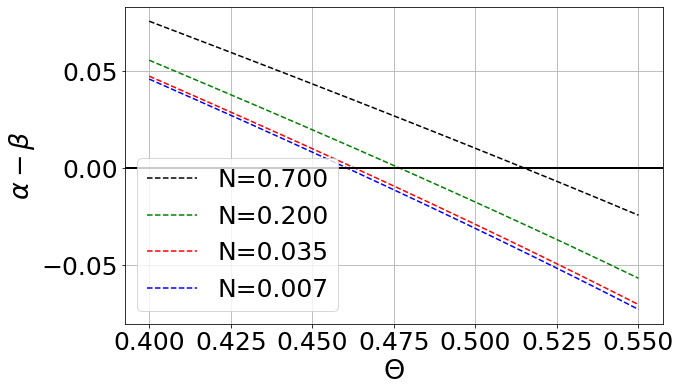
\includegraphics[scale=0.5]{alpha_minus_beta}
    \caption{Evolution of the difference between $\alpha$ and $\beta$ as a
    function of the cut value for different of feed assays, 0.007 (black),
    0.035 (red), 0.2 (green), 0.7 (black). }
    \label{fig_a_m_b}
\end{figure}

From equation \eqref{eq_alpha} and \eqref{eq_beta} it is possible to determine
the cut, $\theta$ required to build an ideal cascade:

\begin{eqnarray}
    \theta_{i} = \dfrac{N_{i} - \dfrac{1}{1 + \beta/R_{i}}}{ \dfrac{\alpha R_{i}}{1 + \alpha R_{i}} -
           \dfrac{1}{1 + \beta/R_{i}}}
           \label{eq_theta}
\end{eqnarray}


As $\alpha_{i}$ and $\beta_{i}$ remain constant, only the value of the cut,
$\theta_{i}$, changes across the different stages of a cascade.  This algorithm
assumes that the corresponding separative power $\delta U$ (not re-computed) can
be achieved with the chosen centrifuge design, tuning other operational
parameter such as the rotation speed, the counter-current flow ratio, etc.  Once
$\theta_{i}$ is determined, it is possible to compute the product and the tail
assay.




The design of the ideal symmetric cascade is performed through 2 steps.  First
one determines the configuration and number of stages, adding stages until the
product assay of the final stage is greater or equal the product targeted assay,
and similarly the tails assay is less or equal the tails desired assay.  This
determines the number of enriching and stripping stages as well as their
enrichment properties ($N_{i}$, $N'_{i}$, $N''_{i}$,$\theta_{i}$i).


The second step determines the relative flows at each stages, solving the linear
flow equation, \eqref{eq_flow}.
The cascade can then be populated with actual machines until the maximum number
available of machines is reached.

\begin{equation}
\setcounter{MaxMatrixCols}{20}
\begin{bmatrix}
     -1      & 1-\theta_{_{S+1}} & 0                 & ...  & 0            & 0            & 0             & 0             & 0             & ... & 0               & 0  & 0 \\
\theta_{_S}  & -1                & 1-\theta_{_{S+2}} & ...  & 0            & 0            & 0             & 0             & 0             & ... & 0               & 0  & 0 \\
             &                   &                   &      &              &              & ...           &               &               &     &                 &    &   \\
 0           & 0                 & 0                 & ...  & \theta_{_-2} & -1           & 1-\theta_{_0} & 0             & 0             & ... & 0               & 0  & 0 \\
 0           & 0                 & 0                 & ...  & 0            & \theta_{_-1} & -1            & 1-\theta_{_1} & 0             & ... & 0               & 0  & 0 \\
 0           & 0                 & 0                 & ...  & 0            & 0            & \theta_{_0}   & -1            & 1-\theta_{_2} & ... & 0               & 0  & 0 \\
             &                   &                   &      &              &              & ...           &               &               &     &                 &    &   \\
 0           & 0                 & 0                 & ...  & 0            & 0            & 0             & 0             & 0             & ... & \theta_{_{E-2}} & -1 & 1-\theta_{_E} \\
 0           & 0                 & 0                 & ...  & 0            & 0            & 0             & 0             & 0             & ... & 0               & \theta_{_{E-1}} & -1
 \end{bmatrix}
 \times
 \begin{bmatrix}
     F_{_{S}}   \\
     F_{_{S+1}} \\
     \cdots     \\
     F_{_{-1}}  \\
     F_{_{0} }  \\
     F_{_{1} }  \\
     \cdots     \\
     F_{_{E-1}} \\
     F_{_{E}}
 \end{bmatrix}
 =
 \begin{bmatrix}
     0      \\
     0      \\
     \cdots \\
     0      \\
     F      \\
     0      \\
     \cdots \\
     0      \\
     0
\end{bmatrix}
%\caption{caption needed!}
\label{eq_flow}
\end{equation}



\subsection{Misuse models}

Little information is available about optimising an existing enrichment cascade
that is being fed with a feed enrichment that does not match the design
enrichment. So far 3 different methods have been investigated.

The first one assumes that no change are been made to the cascade, i.e $\delta
U$, $F$ and $\theta$ are fixed across all stages. The second one assumes the cut
value at each stage is retuned to maintain the ideal state of the cascade,
$\alpha$ and $\beta$ remain fixed. The last one, described in \cite{walker.2017}
assumes the tails to product enriching factor and the cut remain constants ($\gamma =
\alpha\times\beta$). Models behaviors and assumptions are summarized in Tab.
\ref{tab:models}.

\begin{table}[htb]
\centering
  \caption{Summary of misuse model properties.}
\begin{tabular}{l|ccc}
\toprule

Model                &    A                 & B                  & C  \\
\midrule
Constant parameters  & $\alpha_i, \theta_i$ & $\alpha_i=\beta_i$ & $\gamma_i=\alpha_i .\beta_i, \theta_i$       \\
Varying parameters   & $\beta_i$            & $\theta_i$         & $\alpha_i, \beta_i$                     \\
Assays determination & blended              & ideal              & blended                  \\
Flow                 & unchanged            & reduced            & unchanged       \\

\bottomrule
\end{tabular}
  \label{tab:models}
\end{table}


\subsubsection{Model A}

The tuning method A does not re-optimize $\theta_i$ keeping the same flow as the
ideal configuration. From equation \eqref{eq_alpha}, maintaining $\delta U$, $F$
and $\theta$ unchanged implies $\alpha$ remains unchanged as well. According to
equation \eqref{eq_beta}, when $\alpha$ and $\theta$ are fixed, if the feed
assay ($N$) changes, $\beta$ will change accordingly.  This breaks the
ideal status of the cascade, i.e. $N_{i} \neq N'_{i-1} \neq N''_{i+1}$.


In order to compute the proper product and tails assay at each stage, the tails
and the product from the next and the previous stage respectively must be
blended in order to determine the correct stage feed assay. All feed assays are
iteratively updated, blending the proper product and tails, then using the
updated feed assay, the new product and tails assays are recomputed. This
process is repeated until the sum of the square difference in assays is smaller
than $10^{-8}$.  As the cut remain fixed at each stage the flows do not need to
be recomputed.

This model assumes that it is possible to maintain the separative power of a
centrifuges, $\delta U$, for any feed assays $N$ while maintaining its cut
$\theta$ and feed flow $F$.

\subsubsection{Model B}

Using the second method, the cut value at each stage $\theta_i$, is retuned in
order to maintain the $\alpha_i$ and $\beta_i$ at their original values
(equation \eqref{eq_theta}). The cascade remaining ideal, the product and tails
assay at each stages are easily determined using equations \eqref{eq_alphabeta}.

As the cut values change, the relative flow rates between the different stages
are recomputed using equation \eqref{eq_flow}.  Under this model, the flow at
each stage of the original ideal cascade is assumed to be the maximum flow
allowed at that stage.  Therefore, all of the recomputed flow rates are scaled
together to ensure that no stage experiences a flow rate larger than that of
the original cascade.  Some stages may now experience flow rates much lower
than the original cascade.

%% The flow rates are determinted as
%% the largest flow rates allowed by the cascade design, number of centrifuges
%% limiting the flow at each stage.

This model assumes that it is possible to tune a centrifuge separative power
$\delta U$, for any feed assay $N$, cut $\theta$ and feed flow $F$, in order to
maintain its constant feed to product enrichment factor $\alpha$.




\subsubsection{Model C}
The last model assumes that the tails to product enrichment factor remains
constant regardless to the feed assays. To compute the response of the cascade
one need to determine $\alpha$ and $\beta$ such that their product and
$\theta$ remain fixed.
From equations \eqref{eq_alphabeta} and the assay conservation equation $N =
\theta N' + (1-\theta)N''$ it is possible to express the product $N'$ as a function of
the feed assay $N$, $\gamma$ and the cut $\theta$ as one solution of the second
order equation \eqref{eq_gamma_p}:

\begin{equation}\label{eq_gamma_p}
    \theta(\gamma-1)N'^2+((N+\theta)(\gamma-1)+1)N'-N\gamma = 0
\end{equation}


The only solution allowing product assay to range between 0 and 1 is the
following :
\begin{equation}\label{eq_model_b_sol}
    N' = \frac{N+\theta}{2\theta} +
         \frac{1 - \sqrt{\gamma^{2}(N-\theta)^{2}
                         + 2\gamma( N^{2} + N - \theta^{2} + \theta)
                         + (N + \theta + 1)^{2}}}
              {2\theta(\gamma - 1)}
\end{equation}
Once the product assay is known, one can trivially determine the tails assay,
$\alpha$ and $\beta$ using equations \eqref{eq_alphabeta} and mass
conservation.

Similar to model A, because the cut values remain constant, the flows don't
need to be recomputed, and the correct assays, $\alpha$ and $\beta$ are
determined through iterative blending of the product assays of the previous
stage and the tails assay of the next stage using equation
\eqref{eq_model_b_sol}.

This model assumes that it is possible to tune the centrifuge separative power
$\delta U$ in order to maintain, for any feed assay $N$, its tails to product
enrichment factor $\gamma$, while maintaining its cut $\theta$ and feed flow
$F$.

These models inherently result in differing amounts of diminishing returns
as can be seen in Figure \ref{fig:model_comparison}. As the product assay
weight percent increases, the required increase in feed assay to achieve the
same rate of increase grows. This is particularly true for Models A and C
compared to Model B.

\begin{figure}[ht]
    \centering
    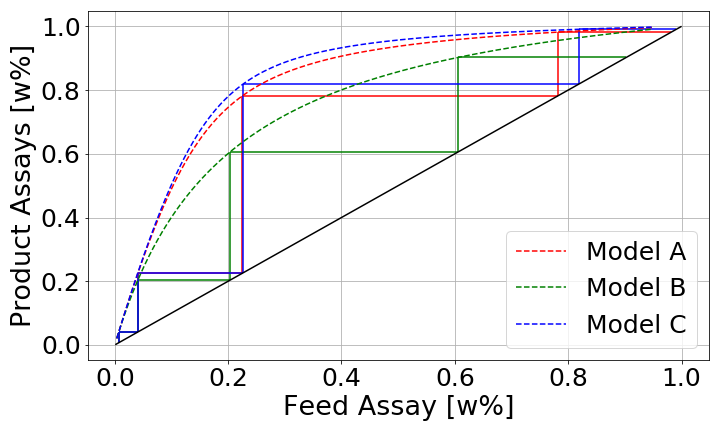
\includegraphics[scale=0.4]{ModelComparison}
    \caption{}
    \label{fig:model_comparison}
\end{figure}
